
\documentclass{include/thesisclass3}

\SelectLanguage{ngerman}
\usepackage{float}


% Titlepage settings
\newcommand{\praktikum}{Praktikum moderne Physik}
\newcommand{\autora}{Jens Schäfer}
\newcommand{\autorb}{Jan van der Linden}
\newcommand{\maila}{ugecd@student.kit.edu}
\newcommand{\mailb}{jan.vdlinden95@gmail.com}
\newcommand{\topic}{Black Lipide Membrane - BLM}
\newcommand{\ptime}{01. Mai 2017}


% Shortcuts
\newcommand{\cc}{\cdot}
\newcommand{\rk}{\rangle}
\newcommand{\lk}{\langle}
\newcommand{\df}{\rightarrow}
\newcommand{\la}{\lambda}
\newcommand{\dd}{{\rm d}}
\newcommand{\ehm}{\mathbbm{1}}
\newcommand{\p}{\partial}
\newcommand{\soll}{\overset{!}{=}}
\newcommand{\D}{\Delta}
\newcommand{\eps}{\epsilon}
\newcommand{\vektor}[3]{\begin{pmatrix} #1 \\ #2 \\ #3 \end{pmatrix}}
\newcommand{\vektorz}[2]{\begin{pmatrix} #1 \\ #2 \end{pmatrix}}
\newcommand{\Mat}[9]{\begin{pmatrix}#1&#2&#3\\#4&#5&#6\\#7&#8&#9\end{pmatrix}}
\newcommand{\Matz}[4]{\begin{pmatrix}#1&#2\\#3&#4\end{pmatrix}}
\newcommand{\e}[1]{\,\si{#1}}
 


\begin{document}

	\FrontMatter
	% coordinates for background border
\newcommand{\diameter}{20}
\newcommand{\xone}{-15}
\newcommand{\xtwo}{160}
\newcommand{\yone}{15}
\newcommand{\ytwo}{-253}




\begin{titlepage}
    % background border
    \begin{tikzpicture}[overlay]
    \draw[color=gray]
            (\xone mm, \yone mm)
      -- (\xtwo mm, \yone mm)
    arc (90:0:\diameter pt)
      -- (\xtwo mm + \diameter pt , \ytwo mm)
        -- (\xone mm + \diameter pt , \ytwo mm)
    arc (270:180:\diameter pt)
        -- (\xone mm, \yone mm);
    \end{tikzpicture}



    % KIT image and sign for faculty of physics
    \begin{textblock}{10}[0,0](4.5,2.5)
        \includegraphics[width=.25\textwidth]{include/kitlogo.pdf}
    \end{textblock}
    

    % horizontal line
    \begin{textblock}{10}[0,0](4.2,3.1)
        \begin{tikzpicture}[overlay]
        \draw[color=gray]
                (\xone mm + 5 mm, -12 mm)
          -- (\xtwo mm + \diameter pt - 5 mm, -12 mm);
        \end{tikzpicture}
    \end{textblock}



    % begin of text part
    \changefont{phv}{m}{n}    % helvetica
    \centering



    % thesis topic (en and ge)
    \vspace*{3cm}
    \Huge\praktikum\\



    % author name and institute
    \vspace*{5cm}
    
    \huge\topic\\






    % examiners (Referenten)
    \vspace*{3cm}
    \Large
    \begin{center}
        \begin{tabular}[ht]{l c l } 
  \autora & \hfill & \textit{\maila} \\
\autorb & \hfill & \textit{\mailb} \\
        
        \end{tabular}
    \end{center}



    % working time
    \vspace{2cm}
    \begin{center}
        \large{Durchgeführt am}: \ptime
    \end{center}



    % lowest text blocks concerning the KIT
    \begin{textblock}{10}[0,0](4,16.8)
        \tiny{KIT -- Universität des Landes Baden-Württemberg und nationales %
              Forschungszentrum in der Helmholtz-Gemeinschaft}
    \end{textblock}
    \begin{textblock}{10}[0,0](14,16.75)
        \large{\textbf{www.kit.edu}}
    \end{textblock}
\end{titlepage}

	\tableofcontents                  
	\newpage
	\MainMatter

%Protokollstart

\chapter{Theoretische Grundlagen}
\section{Ziel des Experiments}
In diesem Experiment soll anhand eines Modells untersucht werden, wie ein Antibiotikum auf eine Zellmembran wirkt. Dazu wird ein Präparat einer Lipid Doppelmembran angefertigt und einem Antibiotikum (Gramicidin A) ausgesetzt. Durch das Antibiotikum werden Ionenkanäle in der Membran gebildet und somit Kationenfluss ermöglicht. Für eine Zelle bedeutet dies, dass ihr Potential zusammenbricht und sie stirbt.\\
\\
Hier soll die Generierung einer solchen Membran beobachtet werden und das Entstehen sowie die Beschaffenheiten der Ionenkanäle näher untersucht werden.


\section{Black Lipid Membran Methode}

Bei der Black Lipid Membran Methode ist eine speziell geformte Küvette aus PTFE Herzstück des Aufbaus. Zwei Tanks werden durch eine Trennwand abgeschirmt die eine kleine, kreisrunde Öffnung mit abgerundeten, weichen Kanten beinhaltet. Eine Wand der Küvette beinhaltet ein Fenster wodurch die Öffnung beobachtet werden kann. In dieser Öffnung werden die Peptide aufgetragen. Sie bilden einen geschlossenen, zunächst undurchdringlichen Film. Die beiden Tanks werden mit Elektrolyten gefüllt und Ag/AgCl-Elektroden ausgestattet. Durch die Zerstörung der Lipidschicht kann nun ein elektrischer Strom die Barriere überwinden und gemessen werden \ref{aufbau}.\\
\begin{figure}[ht]
	\begin{center}
		\includegraphics{images/experiment.png}
		\caption{Experimenteller Aufbau}
		\label{aufbau}
	\end{center}
\end{figure}
Die Natur der Lipide gibt vor, dass sie sich innerhalb einer Grenzschicht parallel anordnen. Dabei zeigen in wässriger Lösung die hydrophilen Köpfe nach außen, nach innen gerichtet sind die hydrophoben Fettsäureketten, die sich mit den Fettsäuren der gegenüberliegenden Grenzschicht anziehen. So bauen die Lipide eine Kette mit einer gewissen Oberflächenspannung auf und trennen die Tanks dicht ab \ref{double}. Die Dicke wird somit ziemlich gut konstant gehalten und die Doppelschicht besitzt isolierende Eigenschaften. Daher kann man die Trennlinie in guter Näherung als Plattenkondensator ansehen.\\
\begin{figure}[ht]
	\begin{center}
		\includegraphics{images/lipid-doublelayer.png}
		\caption{Lipid-Doppelschicht}
	\label{double}
	\end{center}
\end{figure}
Die Dicke der Leptidschicht kann anhand ihrer optischen Eigenschaften eingeordnet werden. Eine weiße Schicht hat eine Dicke d gegenüber der Wellenlänge $\lambda \ll d$, bei $\lambda \approx d$ zeichnen sich newtonsche Ringe ab und für $\lambda \gg d$ erscheint die Oberfläche schwarz. Die Membran wird bei sehr geringer Dicke bevorzugt untersucht um die Kondensatornäherung bestmöglich zu erfüllen und die Bildung von Gramicidin A Kanälen zu gewährleisten.

\section{Gramicidin A}
Gramicidin A ist ein Peptid-Antibiotikum. Diese bestehen in der Regel aus 10 bis 50 Aminosäuren und können mit Zellmembranen interagieren.\\
Im Körper werden Peptid-Antibiotika selbst generiert und werden benutzt, um infizierte Zellen zu zerstören.  Um dies zu bewerkstelligen integrieren sie sich in die Zellmembran und ermöglichen es somit Ionen in die Zelle einzudringen. Bei Gramicidin A geschieht dies durch die Bildung von Kanälen in der Membran. Diese haben Durchmesser von etwa $3 - 4\e{\AA}$. Durch den Fluss von Kationen in die Zelle wird damit ihr elektrochemisches Gleichgewicht gestört und sie stirbt ab.\\
In diesem Experiment wird die Penetration der Zelle durch die Lipid Doppelmembran simuliert; nachdem sich die Membran gebildet hat, ist kein Stromfluss mehr durch die Elektroden möglich. Nach Zugabe von Gramicidin A können in der Membran Kanäle gebildet werden, welche Stromfluss ermöglichen. Dies ist gleichbedeutend mit einer erfolgreichen Bekämpfung und Zerstörung einer infizierten Zelle im Körper mittels eines Peptid-Antibiotikums.


%hab keine lust die verschiedenen penetrationsmethoden zu beschreiben, juckt ja auch keinen.


\section{Generierung der Membran}
Als erster Versuchsschritt soll eine Membran generiert werden. Dazu wird eine geringe Menge an Glycerol Monooleat in Tetradecan auf die Öffnung gebracht. Dadurch wird eine Lipide Doppelmembran generiert. Dies soll optisch beobachtet werden; die Farbe der Membran verändert sich, je nach Dicke bis sie komplett schwarz wird.\\
Für die fertige Membran kann die Leitfähigkeit sowie die Kapazität und die Dicke bestimmt werden. \\Die Leitfähigkeit $G$ kann über den gemessenen Strom durch die Membran und die angelegte Spannung bestimmt werden über $G = \frac{I}{U}$. \\Um die Kapazität zu bestimmen kann angenommen werden, dass die Doppelmembran  sich im Stromkreislauf wie ein Plattenkondenstator verhält. Daher ist der übliche Zusammenhang für einen Plattenkondensator gültig:
\begin{equation}
C = e_0e_m \frac{A}{d}
\end{equation}

% Dicke, spez. Membrankapazität, Membranwiderstand, Durchbruchspannung, max. E-Feld


\section{Einzelkanal Messungen}
Gibt man nur sehr geringe Mengen Gramicidin A in die Lösung so bilden sich auch nur sehr wenige Kanäle in der Membran. Dies wird durch einen quantisierten Stromverlauf sichtbar womit die Anzahl der aktiven Kanäle und auch der Stromfluss pro Kanal bestimmbar sind.\\
Ebenso kann durch die Aufnahme eines Histogramms der ermittelten Lebensdauern die Lebensdauer eines Kanals bestimmt werden, da zu erwarten ist, dass die Lebensdauern exponentiell abfallend verteilt sind.\\
Desweitern gilt zu überprüfen, ob das Ohmsche Gesetz hier erfüllt ist:
\[ I_M = \lambda_M \cc V_M\]
mit $I_M$ dem Strom und $\lambda_M$ der Leitfähigkeit durch die Membran, sowie $V_M$ die Potentialdifferenz der beiden Elektrolyte auf beiden Seiten der Membran.

%Ohms Gesetz

\section{Multikanal Messungen}
Erhöht man die Konzentration des Gramicidin A so öffnen und schließen sich viel mehr Kanäle und eine Vermessung der einzelnen Kanäle ist nicht mehr möglich. Jedoch besteht die Möglichkeit Aussagen über das Öffnen und Schließen der Kanäle, also die Lebenszeit durch eine Autokorrelationsfunktion zu treffen.\\
Dazu soll ein Stromhistogramm aufgenommen werden und über Autokorrelation verglichen werden. Dazu verschiebt man den Verlauf des Histogramms in der Zeit und summiert das Produkt der ursprünglichen und der verschobenen Verteilung binweise auf. Ein hoher ist somit gleichzusetzen mit einer hohen Korrelation der Werte. Der Autokorrelationswert $AC$ einer Funktion $f(t)$ bei einer Verschiebung um $t'$ berechnet sich beispielsweise durch
\[ AC = \frac{1}{T}\sum_t^T f(t)\cc f(t-t') \]
Hier ist für die Strommessung ein exponentieller Abfall des Autokorrelationswertes mit der Zeitverschiebung zu erwarten, da mit steigender Zeitdifferenz die Wahrscheinlichkeit sinkt, dass ein Kanal zu beiden Zeiten geöffnet ist. Ist ein Kanal zu beiden verglichenen Zeiten geöffnet, so trägt dieser zur Korrelation bei. Die mittlere Lebenszeit $\tau$ eines Kanals wird sich demnach als Zerfallskonstante im exponentiellen Abfall widerspiegeln:
\[ AC(t') \sim \exp\left( - \frac{t'}{\tau}\right)\]


\section{Gausssche Fehlerfortpflanzung}
Berechnet sich eine Größe $A$ aus mehreren Größen $x_i$ welche eine statistische Unsicherheit $\sigma_i$ besitzen, so propagiert die Unsicherheit der $x_i$ weiter zu einer Unsicherheit $\sigma_A$ in $A$. Diese Fehlerpropagation wird durch die Gaussche Fehlerfortpflanzug ausgedrückt:
\begin{equation}
\sigma_A = \sqrt{\sum_i \left( \frac{\p A}{\p x_i} \cc \sigma_i \right)^2 }
\label{gauss}
\end{equation}



\chapter{Versuchsauswertung Teil 1}
\section{Auftragen der Membran}
Um die BLM zu Präparieren wurde mit einem Teflonstab ein dünner Film der Peptidschicht auf die Kapilare aufgetragen. Die anfangs dicke Schicht wird durch sanftes abstreifen, klopfen oder rühren verjüngt. Durch die Kamera kann dabei die Ausprägung der newtonschen Ringe beobachten werden. In Abbildung \ref{Reihe} ist Kapilare mit unterschiedlich dicken Lipidmembranen zu sehen. Links ist die Membran dick genug, um Licht hindurch zu lassen, sie erscheint durchsichtig. Die mittlere ist im Bereich der Wellenlängen von sichtbarem Licht und bildet damit newtonsche Ringe aus. Bei der dritten Aufnahme ist die Membran im Begriff sich auszudünnen, man erkennt die Lichtunterdrückung rechtsseitig und damit die Schwarzfärbung.
\begin{figure}[H]
	\begin{center}
		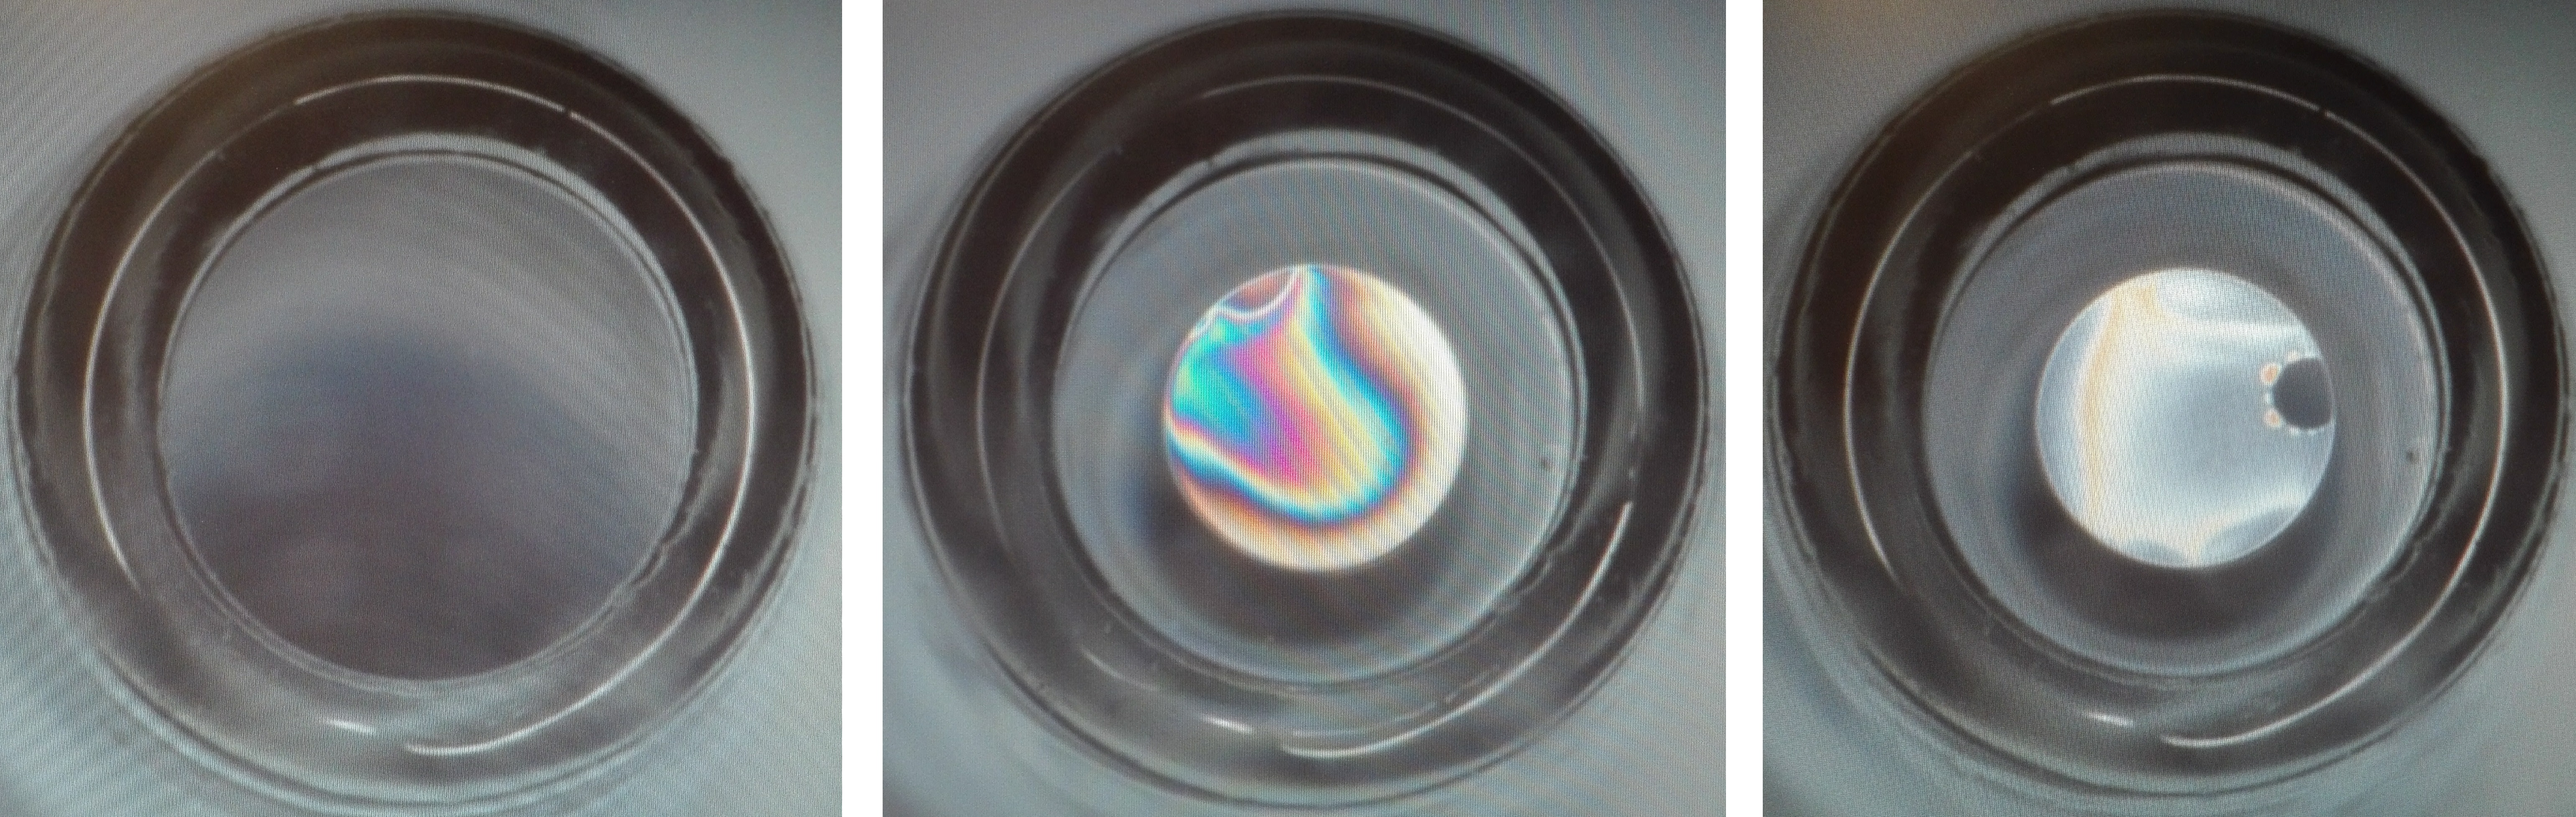
\includegraphics[width=1\textwidth]{images/Reihe.png}
		\caption{Lichtdurchlässige Membran (l), Newtonsche Ringe (m), BLM (r)}
		\label{Reihe}
	\end{center}
\end{figure}
\section{Membranfläche}
Um die Fläche der Membran zu bestimmen wurden die Kameraaufnahmen untersucht. Relevant für die untersuchten Prozesse ist nur jener dünne und schwarze Anteil der Membran. Hierzu dient die Aufnahme \ref{Perle}. Bei der Untersuchung der Verhältnisse aus Pixel/Milimeter für den Kapilaraußen/ und -innendurchmesser fällt auf, dass das Verhältniss mit zunehmendem Abstand von der optischen Achse zunimmt. Dieser Effekt ist der Krümmung der Linse verschuldet und wird in der Optik als kissenförmige Verzeichnung bezeichnet \ref{Verzeichung}.
\begin{figure}[h]
	\begin{center}
		\includegraphics[width=0.3\textwidth]{images/Verzeichnung.png}
		[\url{https://upload.wikimedia.org/wikipedia/commons/0/0a/Verzeichnung3.png}]
		\caption{Kissenförmige Verzeichnung durch die Krümmung der Linse}
		\label{Verzeichnung}
	\end{center}
\end{figure}
Da die Verzeichnung allerdings exponentiell mit dem Abstand zur Bildmitte zunimmt und die Verhältnisse zwischen Außen- und Innenwand nur 5,59\% (\ref{tab-ratio}) betragen, können im inneren der Kapillare lineare Verhältnisse vorausgesetzt werden, insbesondere da die BLM recht zentriert in der Kapillare auftreten.
Um den Fehler minimal zu halten, rechnet man mit dem Verhältnis des Innendurchmessers um den BLM-Durchmesser zu bestimmen. Dabei sei das Verhältnis Pixeln zu Milimetern im inneren mit 5,59\% grob abgeschätzt. Die Zahlen sind in Tabelle \ref{tab-ratio} eingetragen.

\begin{table}[H]
	\centering
	\begin{tabular}{llll}
		& Au\ss en   & Innen     & BLM     \\
		\O  [Pixel] & 2085    & 1465    & 441     \\
		\O  [Milimeter]       & 1.55    & 1.15    & $\approx$ 0.346   \\
		Verhältnis [p/mm]            & 1345.16 & 1273.91 & $\approx$ 1273.91
	\end{tabular}
	\begin{tabular}{rll}
Verhältniss Außen: & 1345.16\e{\frac{p}{mm}} & \\
Verhältniss Innen: & 1273.91\e{\frac{p}{mm}} & \\
Abweichung: & 71.3 & =~~5.59\%\\
\end{tabular}
	\caption{Vermessung von Kapilare und BLM}
	\label{tab-ratio}
\end{table}

\begin{figure}[ht]
	\begin{center}
		\includegraphics[width=0.4\textwidth]{images/Perle2.png}
		\caption{Vermessung von Kapilare und BLM}
		\label{Perle}
	\end{center}
\end{figure}
Wir gehen also von einem Verhältnis V = (1273.91 $\pm$ 5,59\%) p/mm und einem Durchmesser von (441 $\pm$ 0)p aus. Die Pixel kann mit entsprechender Analysesoftware exakt abzählen. Die Fläche der BLM berechnet sich wie folgt. Der Fehler berechnet sich mit Gau\ss'scher Fehlerfortpflanzung \ref{gauss}:
\begin{equation}
A=\frac{\pi}{4}\cdot 441p/ V=0.0941\e{mm^2}
\end{equation}
\begin{equation}
\Delta A=0.00526\e{mm^2}
\end{equation}

\section{Kapazität}
Bei der Messung der Kapazität wird eine Rechteckspannung von $U_{C0}=5\e{mV}$ mit $f=50\e{Hz}$ an die Elektroden angelegt. Dabei wird ein Widerstand $R_1=100\e{k\Omega}$ in Reihe geschalten und die Spannung über der Membran aufgezeichnet. Abbildung \ref{oszi} zeigt die zugehörige Oszilloskopaufnahme, auf der man die Analogie zum Kondensator verifizieren kann. Eingezeichnet wurde die Peakspannung von $U_0 = 7.5\e{V}$ und die geometrisch konstruierte Strecke von 53 Pixel (hier schätzen wir den Fehler auf $\pm$ 20\%), die der charakteristischen Zeit $\tau$ entspricht, während der die Spannung auf $U_0/\textit{e}\approx 2.8$ abfällt. Daraus lässt sich die Zeit Tau bestimmen und die Kapazität berechnen. Dazu benützen wir das Verhältnis V aus Pixel über Spannung mit V=(1250$\pm$7\%)p/0.02s. Den Fehler auf das Pixelverhältnis haben wir hier höher geschätzt als es aus Abbildung \ref{Perle} ersichtlich wäre, da wir hier keine Referenzwerte zur Abmessung haben. Vorgeschalten wurde der Widerstand R$_1=100\e{k\Omega}$.
\begin{align}
C=\tau/ R_1 = 0.02\e{s}\cdot 53 V/R_1 = (8.48 \pm 1.8)\e{nF}
\end{align}
\begin{figure}[ht]
	\begin{center}
		\includegraphics[width=0.7\textwidth]{images/measure.png}
		\caption{Oszilloskopaufnahme der Entladung der Membran über eine Wechselspannung}
		\label{oszi}
	\end{center}
\end{figure}

\section{Dicke}
Die Dicke der Membran bekommt man aus der Analogie zum Plattenkondensator:
\begin{align*}
	d&=\epsilon_0\epsilon_M \frac{A}{C}\\
	d&=(196.5 \pm 43)\e{nm} \ll \lambda
\end{align*}
Hierbei wurde die Membran aus Abbildung \ref{Perle} untersucht, deren Fläche und Kapazität oben bereits berechnet wurde. 

\section{spezifische Kapazität}
\begin{align}
C_{Spez}=C/A=(9.01 \pm 1.97)\e{\frac{\mu F}{cm^2}}
\end{align}
\section{Durchbruchspannung, maximales E-Feld, Aufnahmequalität}
Aufgrund der schwierigen Bedingungen die an das Labor gestellt werden um eine BLM stabil zu halten, war es vor Ort nicht möglich, alle Messungen durchzuführen. Auch die Aufnahme Abbildung \ref{oszi} konnte in Eile nicht mit höherer Qualität durchgeführt werden, bevor die BLM zerreist.\\
Um die Durchbruchspannung zu bestimmen, hätte man auf eine BLM eine Wechselspannung von zunehmender Stärke angelegt und den Wert für den Durchbruch bestimmt. Das maximale elektrische Feld im Kondensator hätte sich zu $E_{Max}=U_{Durchbruch}/d$ berechnet.
\section{Widerstand}
\begin{figure}[ht]
	\begin{center}
		\includegraphics[width=0.7\textwidth]{images/Widerstand.png}
		\caption{Widerstandsmessung}
		\label{resistance}
	\end{center}
\end{figure}
Um den Widerstand der Membran zu Messen, wurde eine Gleichspannung von $U_0=(15 \pm 10\%)\e{mV}$ angelegt und der Spannungsabfall $U_M$ über der Membran gemessen \ref{resistance}. Mit geschalten waren der Verstärker V=200 und der Vorwiderstand $R_x=500\text{M}\Omega$. Es wird wieder mit dem Verhältnis V$_p=5.77 \pm 7\% \e{\frac{p}{mV}}$ gerechnet.
\begin{align*}
	U_M&= 105\e{p}/V_p= 2.7 e{mV}\\
	R_M&=R_x V U_0 /U_M\\
	R_M&=(82.4 \pm 10.1)\e{G\Omega}
\end{align*}

\chapter{Versuchsauswertung Teil 2}
Im zweiten Teil des Versuchs sollte der Effekt des Antibiotikums Gramicidin A auf die BLM untersucht werden. Da die Generierung einer stabilem BLM jedoch nicht möglich war wird für die folgende Auswertung auf einen Beispieldatensatz der Messungen zurückgegriffen.

\section{Stromfluss durch einen einzelnen Kanal}
Bei einer niedrigen Konzentration an Gramicidin A im Elektrolyt bilden sich in der Membran nur wenige Kanäle, daher ist die Quantisierung des Ionenstroms durch den Kanal gut erkennbar. In Abbildung \ref{singlechannel} ist ein Ausschnitt der Messung des Stroms $I$ über der Zeit dargestellt.
\begin{figure}[H]
\centering
\includegraphics[scale=0.7]{images/ssingle_channel.pdf}
\caption{\textbf{Ausschnitt der Messungen des Durchflussstroms über der Zeit.} Zu erkennen sind niedrige und hohe Plateaus, wobei die niedrigen einem Grundstrom von etwa 3 pA entsprechen. Zur besseren Identifizierung der hohen und niedrigen Plateaus wurden die Messdaten über 20 Messpunkte geglättet. Die hohen Plateaus entsprechen der Öffnung eines einzelnen Kanals wodurch etwa 2 pA zusätzlich fließen. Bei $t = 218\e{s}$ sind für kurze Zeit zwei Kanäle geöffnet, der Strom beträgt dort etwa 6 pA.}
\label{singlechannel}
\end{figure}
Insgesamt wurden über einen Zeitraum von $500\e{s}$ mit einer Frequenz von $50\e{Hz}$ Strommessungen durchgeführt. Für eine genauere Auswertung des Stromflusses durch einen einzelnen Kanal wurden die Stromwerten in Abbildung \ref{singlehist} histogrammiert um die Mittelwerte des Grundstroms, sowie der ersten und zweiten Anregung zu bestimmen.

\begin{figure}[H]
\centering
\includegraphics[scale=0.7]{images/single_hist.pdf}
\caption{\textbf{Histogrammierung der Stromwerte.} Zu sehen sind drei ausgebildete Peaks. Der erste entspricht dem Grundstrom, der zweite entspricht einer Öffnung von einem einzelnen Kanal, der dritte enspricht der Öffnung von zwei Kanälen zur gleichen Zeit. Bei etwa 8 pA ist ein weiterer verlaufener Peak zu sehen, der zur Auswertung jedoch nicht beachtet wurde. Für jeden Peak wurde ein Fit an eine Gaussfunktion durchgeführt und der Mittelwert $\mu$ sowie die Standardabweichung $\sigma$ dargestellt und in Tabelle \ref{singlefits} zusammengefasst. Für jeden Bin wurde ein poissonverteilter Fehler angenommen.}
\label{singlehist}
\end{figure}
\begin{table}[H]
\centering
\caption{\textbf{Fitergebnisse}}
\label{singlefits}
\begin{tabular}{rl}
\toprule
Grundstrom $I_0$ & $(2.75 \pm 0.47)\e{pA}$\\
ein Kanal $I_1$ & $(4.39 \pm 0.57)\e{pA}$\\
zwei Kanäle $I_2$ & $(6.05\pm 0.46)\e{pA}$\\
\bottomrule
\end{tabular}
\end{table}
Der Einzelkanalstrom berechnet sich somit aus der Differenz zweier benachbarter Peaks:
\[
I_{Kanal} = \frac{I_1-I_0}{2} + \frac{I_2-I_1}{2} = 1.65\e{pA}\]
Da die Kanalströme fluktuieren und die Messung der Ströme nur beschränkt genau möglich ist haben die Peaks in Abbildung \ref{singlehist} eine Breite, charakterisiert durch die Standardabweichungen $\sigma$. Diese Unsicherheiten pflanzen sich statistisch in $I_{Kanal}$ fort. Mit Gauss'scher Fehlerfortpflanzung (vgl. Gleichung \ref{gauss}) berechnet sich somit für $I_{Kanal}$ eine statistische Unsicherheit von $\sigma_{Kanal} = 0.33\e{pA}$. Zusammenfassend beträgt der Strom durch einen einzelnen Gramicidin A Kanal somit
\[ I_{Kanal} = (1.65 \pm 0.33)\e{pA}\]

\section{Einzelkanal-Leitfähigkeit}
% 50mV als Generator Spannung nicht sicher.
Durch die Berechnung des Einzelkanal-Stroms $I_{Kanal}$ kann die Leitfähigkeit $\lambda$ eines Kanals bestimmen werden:
\[ \lambda = \frac{I_{Kanal}}{U_{Gen}}\]
Für eine Generatorspannung von $50\e{mV}$ errechnet sich eine Leitfähigkeit von $\lambda = 33.0\e{pS}$.\\
Da für die Generatorspannung keine statistische Schwankung bekannt ist, propagiert allein die Unsicherheit von $I_{Kanal}$ nach $\lambda$. Mit Gauss'scher Fehlerfortpflanzung (vgl. Gleichung \ref{gauss}) ergibt dies $\sigma_\lambda = 6.6\e{pS}$. Zusammenfassend beträgt die Leitfähigkeit eines Gramicidin A Kanals somit
\[\lambda = (33.0 \pm 6.6)\e{pS}\]



\section{Kanalöffnungszeit - Einzelkanalvermessung}
Bei einer niedrigen Konzentration an Gramicidin A ist es möglich, die Lebensdauer eines einzelnen Kanals aus dem Stromdiagramm zu bestimmen, da die Quantisierung der Stromwerte deutlich sichtbar ist. In Abbildung \ref{quant} ist dies verstärkt dargestellt.

\begin{figure}[H]
\centering
\includegraphics[scale=0.7]{images/quantisierung.pdf}
\caption{\textbf{Geglätteter Stromverlauf} für die Einzelkanalmessung im Bereich $80\e{s}$ bis $220\e{s}$. Aus den  Ergebnissen aus Tabelle \ref{singlefits} wurden die Messdaten quantisiert dargestellt. Aus diesen quantisierten Daten konnte die Lebenszeit eines Kanals approximativ über die Breite eines Plateaus bestimmt werden.}
\label{quant}
\end{figure}
Die berechneten Lebensdauern des kompletten Messzeitraums wurden in Abbildung \ref{poiss} histogrammiert dargestellt und mit einer Exponentialfunktion gefittet. 
\begin{figure}[H]
\centering
\includegraphics[scale=0.7]{images/poiss.pdf}
\caption{\textbf{Histogramm der Lebensdauern} der Einzelkanal Messung. Die Fehler auf die Zählrate wurde als poissonverteilt angenommen.}
\label{poiss}
\end{figure}
Durch die Vermessung der Einzelkanäle ergibt sich eine mittlere Lebenszeit von
\[ \tau = p_1 = (0.78 \pm 0.08)\e{s}\]
Generell wird diese Methode der Bestimmung der Lebenszeit als sehr ungenau und fehleranfällig eingeschätzt, da Schwankungen im Strom als Öffnen oder Schließen eines Kanals fehlinterpretiert werden können und bei der Häufung mehrerer offener Kanäle keine Aussage gemacht werden kann, welcher Kanal sich zuerst schließt. 


\section{Kanalöffnungszeit - Multikanalvermessung}
Durch die Zugabe einer höheren Konzentration Gramicidin A zum Elektrolyt bilden sich mehr Kanäle an der Membran. Damit sind zu jeder Zeit mehrere Kanäle offen und es kann keine Analyse der Öffnungs- und Schließzeiten der einzelnen Kanäle anhand des $I-t-$Diagramms durchgeführt werden. \\In Abbildung \ref{multi} ist der Stromverlauf für eine hohe Gramicidin A Konzentration über der Zeit aufgetragen.
\begin{figure}[H]
\centering
\includegraphics[scale=0.7]{images/multi.pdf}
\caption{\textbf{Stromverlauf der Multikanalmessung.} Gemessen wurde ein Zeitraum von $320\e{s}$ mit einer Frequenz von $50\e{Hz}$. Bis $t = 250\e{s}$ ist der Verlauf relativ gleichmäßig; der Strom scheint einen gleichmäßgen Mittelwert von etwa $5\e{pA}$ zu haben, was bedeutet, dass zu jedem Zeitpunkt im Mittel gleich viele Kanäle geöffnet sind. Die Schwankungen um diesen Mittelwert entsprechen dem zufälligen Öffnen und Schließen von Kanälen. Für die weitere Analyse wurde für die Stromwerte ein Fehler von $2 \%$ angenommen.}
\label{multi}
\end{figure}
Aufgrund von starken Ausreißern am Anfang und einem Abfall des Strom-Mittelwerts am Ende wurde für die weitere Analyse nur der Bereich von $60\e{s}$ bis $250\e{s}$ verwendet. In diesem Intervall ist der Mittelwert relativ konstant $\mu = 5.362\e{pA}$. Um die Autokorrelation durchzuführen wurde der Mittelwert von jedem der Werte abgezogen. In Abbildung \ref{AC} ist der Verlauf der Autokorrelationsfunktion für Zeitverschiebungen von $0\e{s}$ bis $4\e{s}$ dargestellt. Für höhere Zeiten beginnt die Autokorrelation zu fluktuieren, daher wurde nur dieser Bereich für die Auswertung berücksichtigt.


\begin{figure}[H]
\centering
\includegraphics[scale=0.7]{images/AC.pdf}
\caption{\textbf{Autokorrelationsfunktion und exponentieller Fit.} Zu sehen ist, dass der Verlauf der Autokorrelationsfunktion nicht exakt einem exponentiellen Zerfall entspricht, was möglicherweise auf systematische Unsicherheiten der Messung zurückzuführen ist. Die statistischen Unsicherheiten der Autokorrelationsfunktion propagierten durch Gauss'sche Fehlerfortpflanzung aus den Strommessungen dargestellt in Abbildung \ref{multi}. }
\label{AC}
\end{figure}
Aus dem exponentiellen Fit der Autokorrelationsfunktion wurde die mittlere Lebensdauer (Zerfallskonstante) eines Kanals zu $\tau = p_1 = (1.10 \pm 0.01)\e{s}$ berechnet.\\
Im Vergleich dieses Ergebnisses mit dem Ergebnis der Einzelkanalvermessung fällt die Unsicherheit viel geringer aus, da die Messstatistik durch die Erhöhung der Kanalmenge stark steigt. Dadurch erzielt diese Messmethode ein genaueres Ergebnis und beruht nicht auf der Abmessung einzelner Plateaubreiten im $I-t-$Diagramm. Dennoch haben beide Ergebnisse die gleiche Größenordnung, was zusätzlich zu einer Vailidierung der Ergebnisse führt.
\end{document}
